
\subsection{Precipitation}
\subsubsection{Annual Mean Anomaly}

\begin{figure}[H]
	\centering
	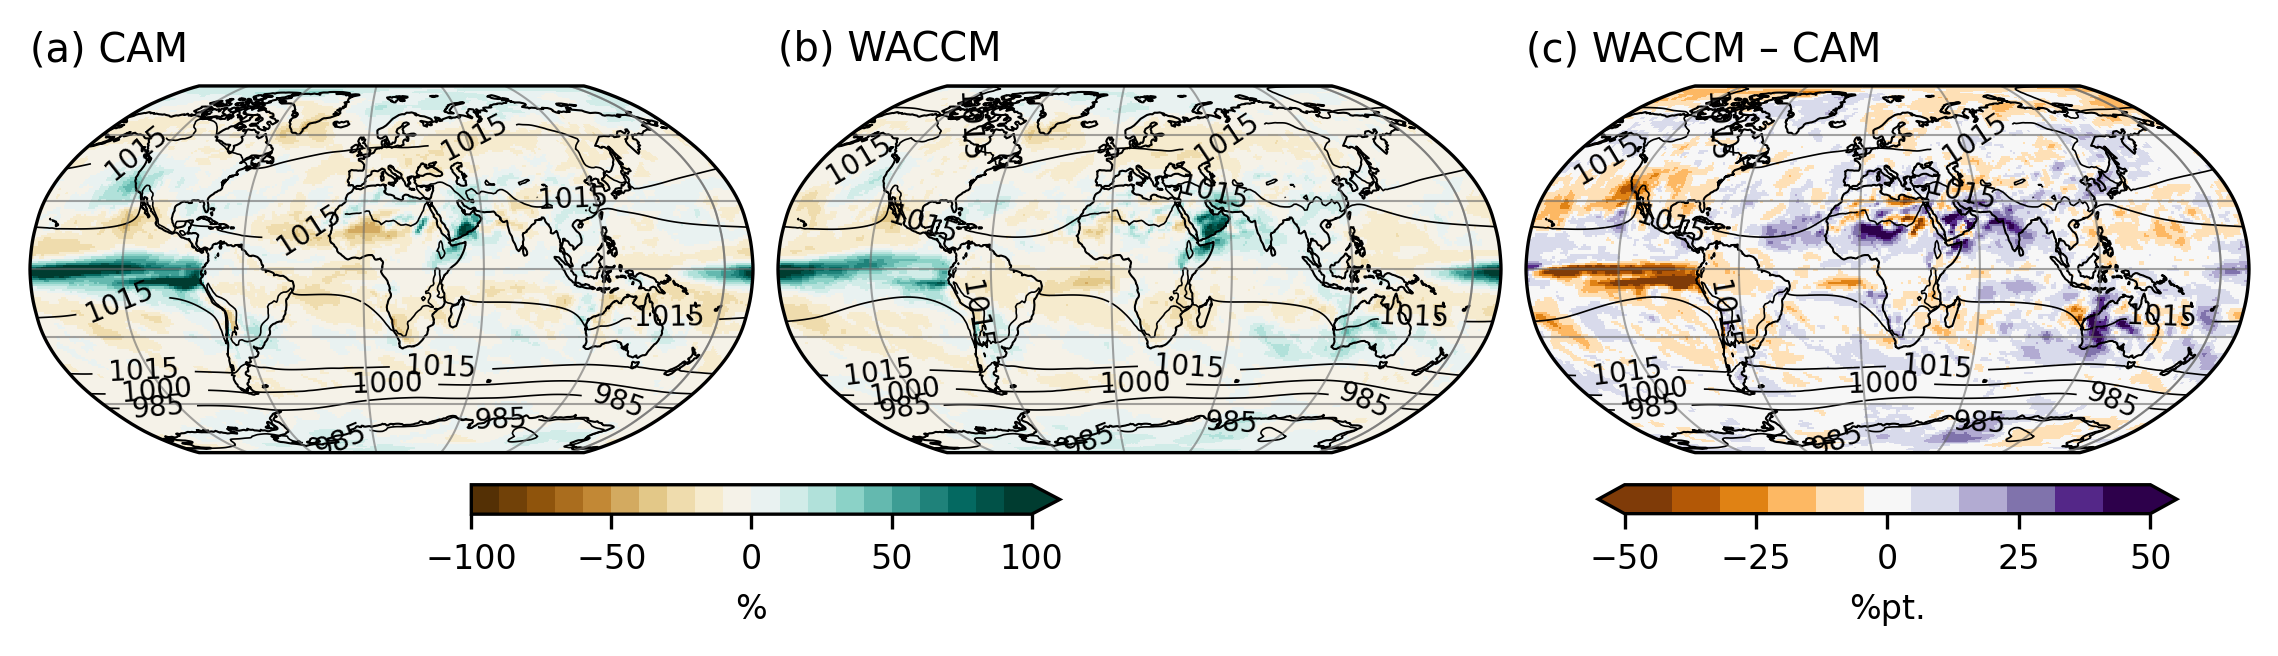
\includegraphics[width=\linewidth]{/Users/Simone/Documents/Uni/Master/Y2/Thesis/Paper_imgs/png/PRECT_ann.png}
	\caption{Annual mean precipitation anomalies of 2080-2099 SAI2020 scenario compared to 2016-2035 Control scenario in (a) CAM and (b) WACCM. Difference between precipiation anomalies shown in (c). 2016-2035 Control sea level pressure shown in black contours.}
	\label{fig:PRECT_ann}
\end{figure}

The annual mean precipitation anomalies are shown in Figure \ref{fig:PRECT_ann}, we learn:

\begin{itemize}
	\item Most areas in both CAM and WACCM follow `wet gets wetter, dry gets drier'.
	\item CAM seems to have an overly active ITCZ over the pacific, though the pattern is similar to WACCM. 
	\item Southern Arabic peninsula and Horn of Africa show similar patterns, now with WACCM showing higher increase in precipitation. 
\end{itemize}

TO DO:
\begin{itemize}
	\item check slp contours/gooi ze weg, voeg reference neerslag toe
	\item min/max aanpassen? ITCZ wordt wel raar
\end{itemize}

\subsubsection{JJA and DJF Seasonal Mean Anomaly}

\begin{figure}[H]
	\centering
	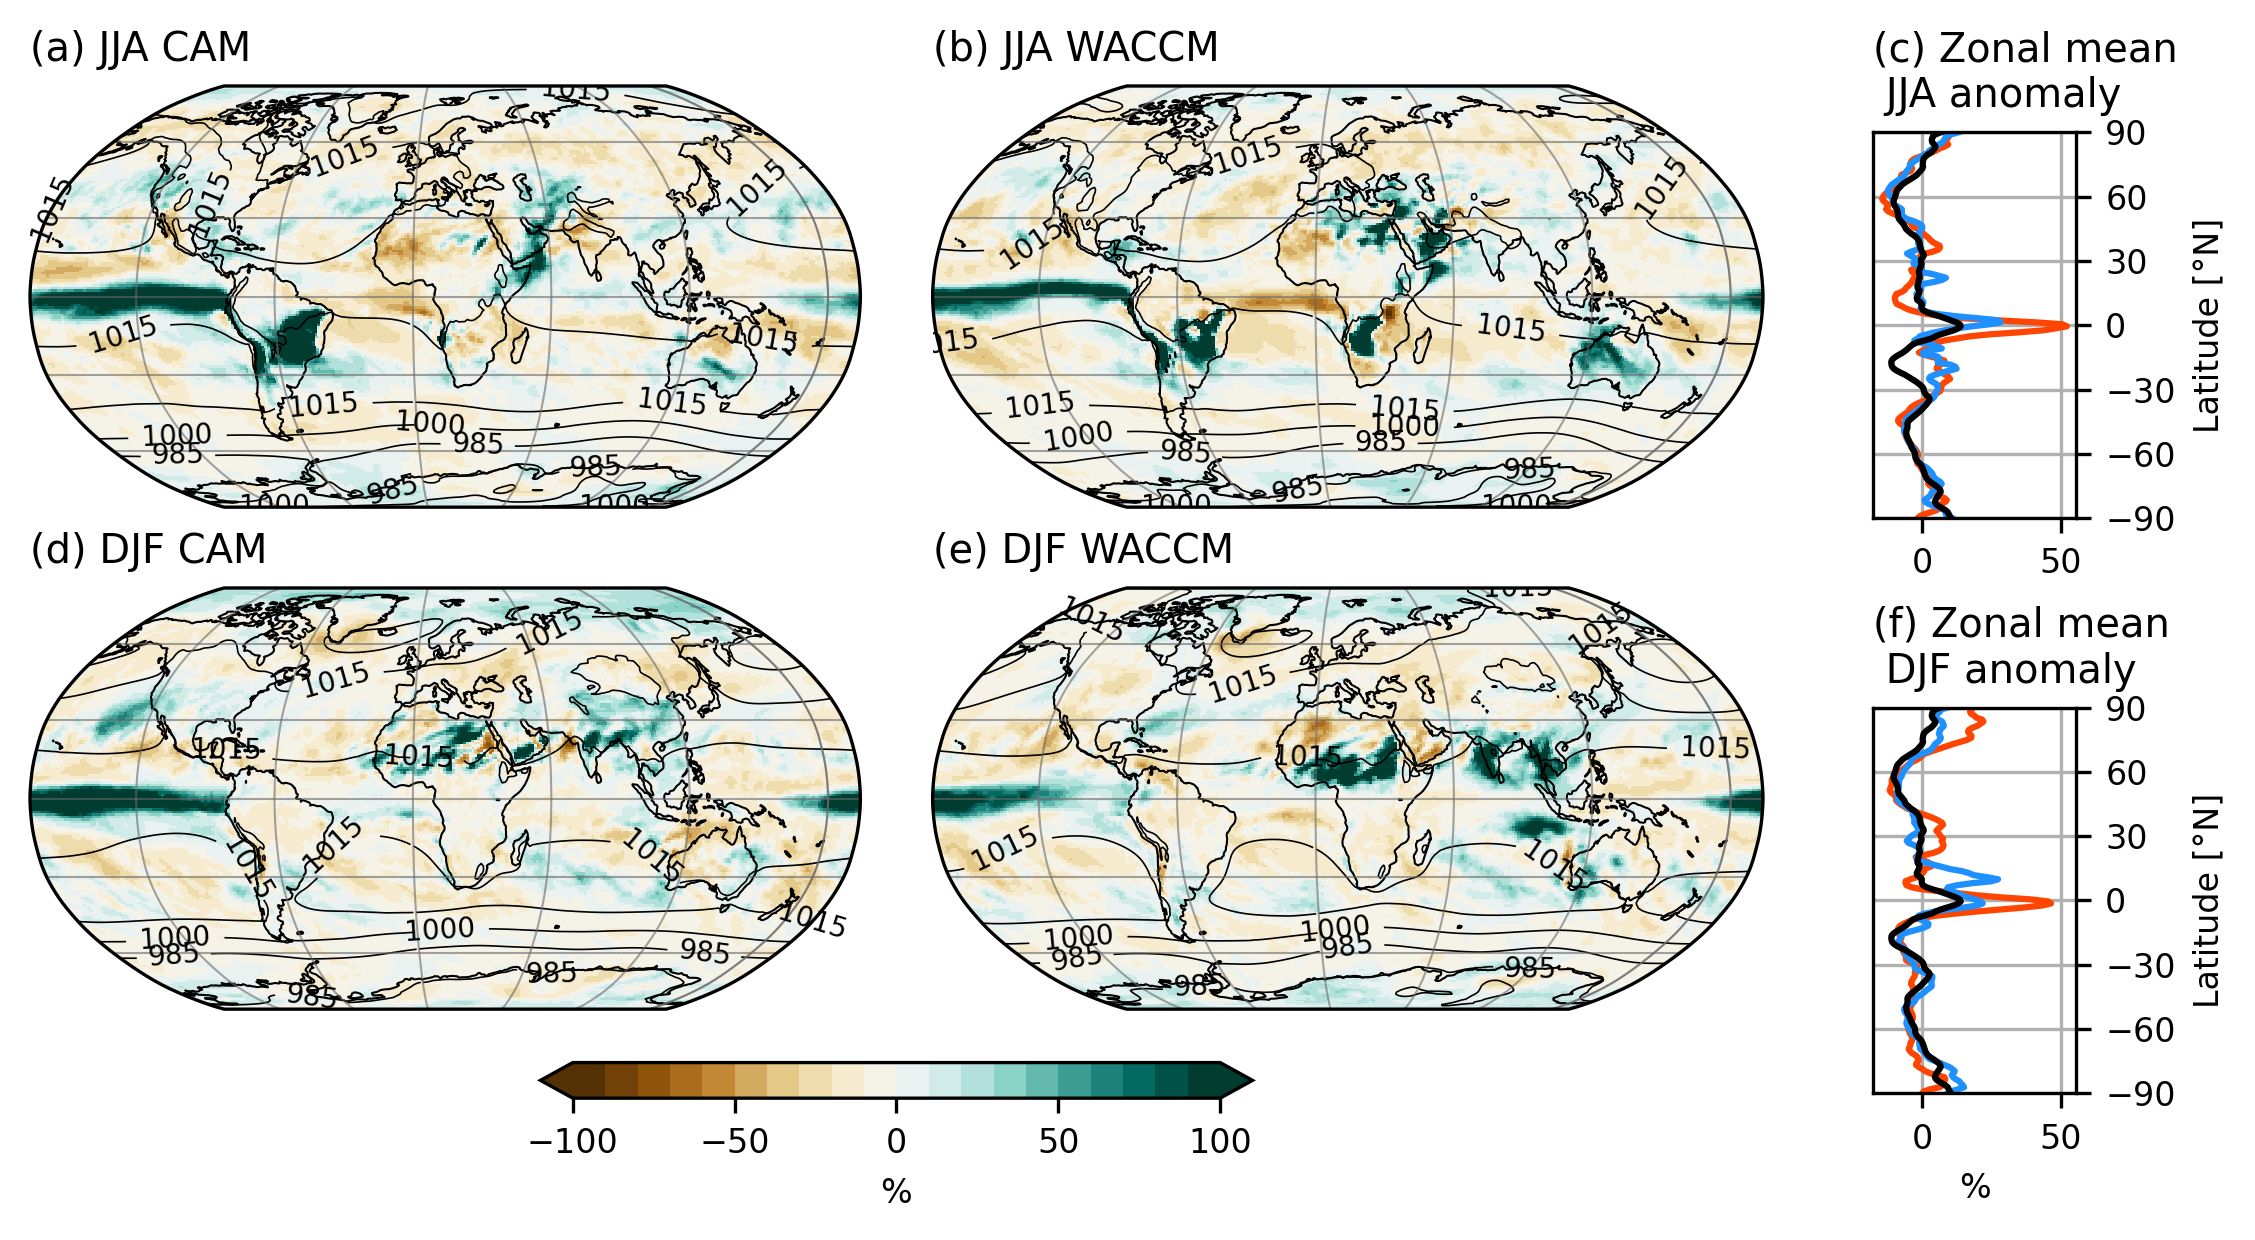
\includegraphics[width=\linewidth]{/Users/Simone/Documents/Uni/Master/Y2/Thesis/Paper_imgs/png/PRECT_seas.png}
	\caption{JJA and DJF seasonal mean precipitation anomalies of 2080-2099 SAI2020 scenario compared to 2016-2035 control scenario in (a),(d) CAM and (b),(e) WACCM. 2016-2035 Control mean sea level pressure shown in black contours. Zonal mean precipitation anomalies shown in (c) and (f)}
	\label{fig:PRECT_seas}
\end{figure}

The JJA and DJF seasonal mean precipitation anomalies are shown in Figure \ref{fig:PRECT_seas} we learn:

\begin{itemize}
	\item In \textbf{JJA} the ITCZ over the pacific is again overly active in CAM, though again showing a similar pattern to WACCM. \item The higher intensity but similar pattern is also clearly visible in the zonal mean anomaly. 
	\item WACCM shows large spots of more than doubling of rainfall in Brazil and Southern Africa, not very significant still because these areas receive very little rainfall. Same goes for the increase in Australia.
	\item In \textbf{DJF} the ICTZ is even more anomalous in CAM than it is in WACCM, now not showing too similar patterns anymore, mainly not increasing in WACCM in the East Pacific. 
	\item In the Sahara region both WACCM and CAM show patches of doubling precipitation, again this is not significant as this area receives very little rainfall. 
	\item WACCM shows a more intense monsoon in Southern and South-East Asia, whereas CAM shows more limited increase in rainfall in Southern Asia. 
	\item The zonal mean anomaly shows that the Arctic is much wetter in CAM. 
\end{itemize}

TO DO:
\begin{itemize}
	\item figure out legend
	\item Why: is WACCM more sensitive for precipitation?
	\item waar regen niet significant is: arcering en/of weglaten?
\end{itemize}